\section{Non-SD Background}\label{section:star_nonSD}
The background contributions coming from \ac{ND}, \ac{DD} and \ac{CD} events are estimated from \ac{MC} simulations. Protons from elastic interactions and beam halo are not included in the~simulation. \ac{SD} background signatures which are modeled in th~\ac{MC} simulations are only coming from :
\begin{itemize}
	\item forward protons produced in the \ac{SD}, \ac{CD} or \ac{DD} diffractive systems or through non-diffractive  \ac{QCD},
	\item reconstructed tracks coming from showering.
\end{itemize}

Figure~\ref{fig:nonSDxit} shows the uncorrected $\xi$ and $t$ distributions in data compared to various \ac{MC} models: PYTHIA 8 A2 (MBR), PYTHIA 8 A2 (MBR-tuned) and EPOS. The \ac{MC} distributions are split into \ac{SD}, \ac{ND}, \ac{DD} and \ac{CD} components. For EPOS low mass excitation of the proton remnant (SD') is separated from the ND events. Additionally, the accidental background is also shown. Without arbitrary suppression of diffractive cross sections at large $\xi$ PYTHIA8 A2 (MBR-tuned) predictions agree much better with the data and result also in a suppression of non-SD events. EPOS describes data better than PYTHIA8 but shows a dominant contribution of SD' events. All MCs predict significant non-SD background at large $\xi$, thereby  the analysis was limited to $\xi < 0.2$. 

On the other hand, \cref{fig:nonSDnsel,fig:nonSDpt,fig:nonSDera} show the uncorrected distributions of variables used in the later analysis: $n_{\mathrm{sel}}$, $p_{\mathrm T}$ an $\bar{\eta}$. The background contributions from non-SD interactions differ a bit between each other, i.e. EPOS predicts significantly larger CD contribution, whereas DD and ND are suppressed in PYTHIA 8 A2 (MBR-tuned).  As a result PYTHIA~8~A2~(MBR) is used as the default model  of non-SD with systematic uncertainty $\pm50\%$, which covers all differences between the~models. %Moreover, SD' in EPOS was not subtracted but used separately for comparisons.

\thispagestyle{empty}
\begin{figure}[h!]
	%\vspace{-0.5cm}
	\centering
	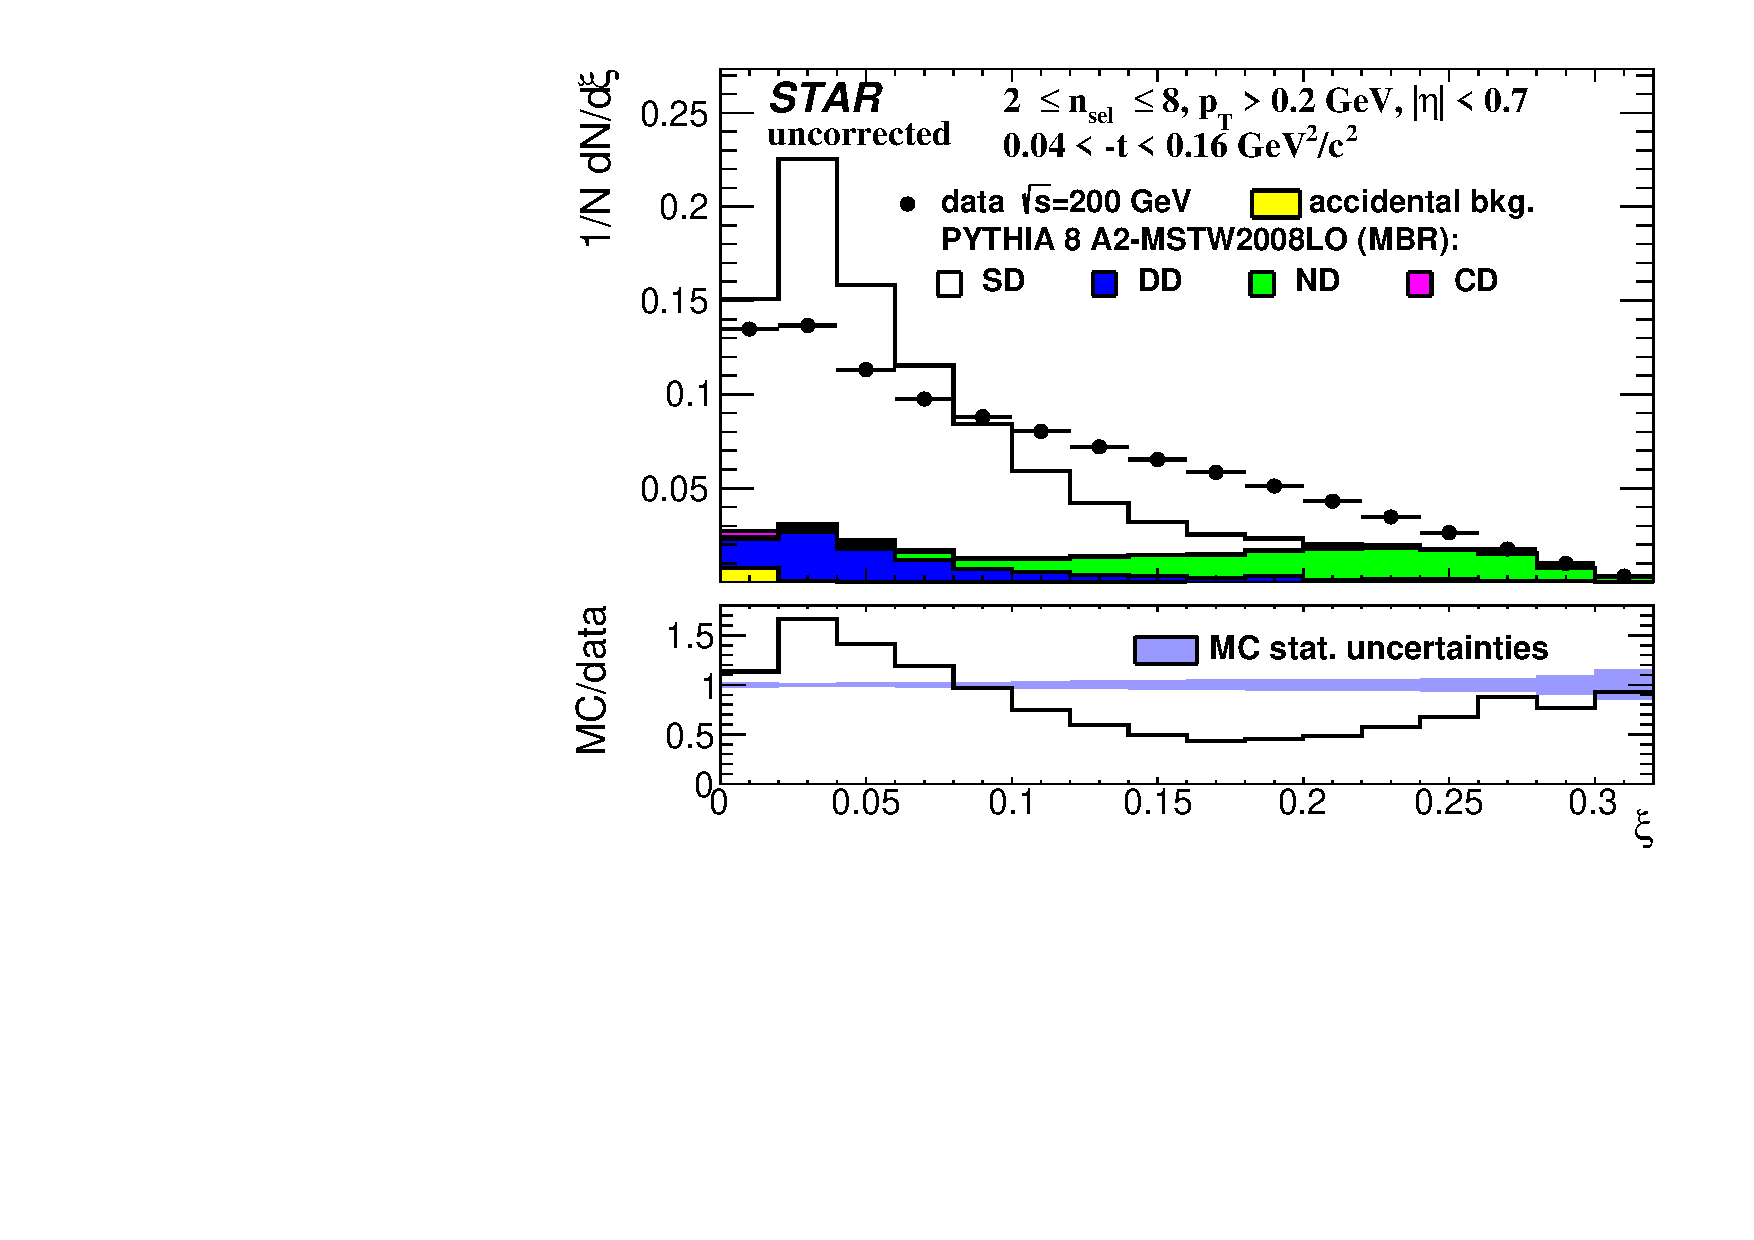
\includegraphics[width=.49\textwidth,page=1]{chapters/chrgSTAR/img/nonSD/SDT_pythia_xi0_RP_starsim_xi.pdf}
	\hfill
	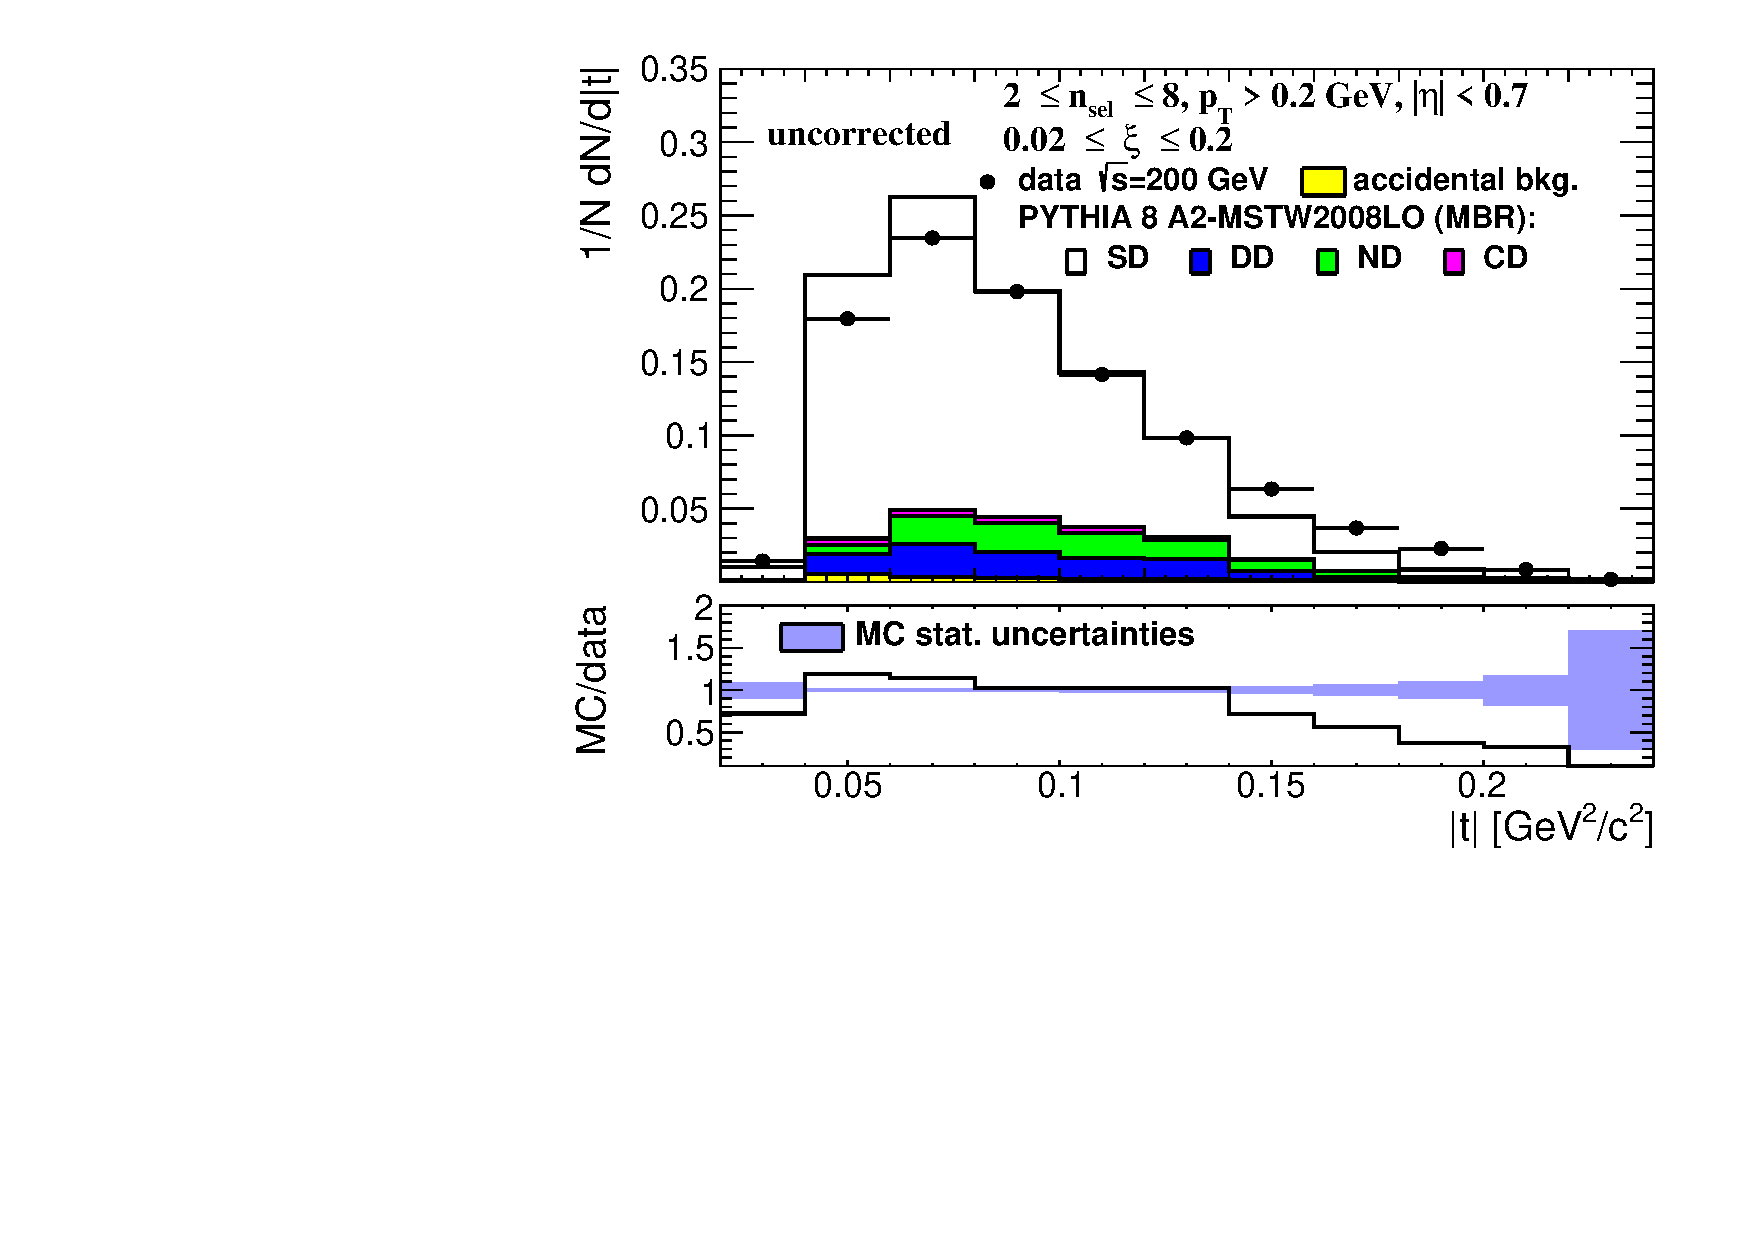
\includegraphics[width=.49\textwidth,page=1]{chapters/chrgSTAR/img/nonSD/SDT_pythia_xi0_RP_starsim_t.pdf}
	\newline
	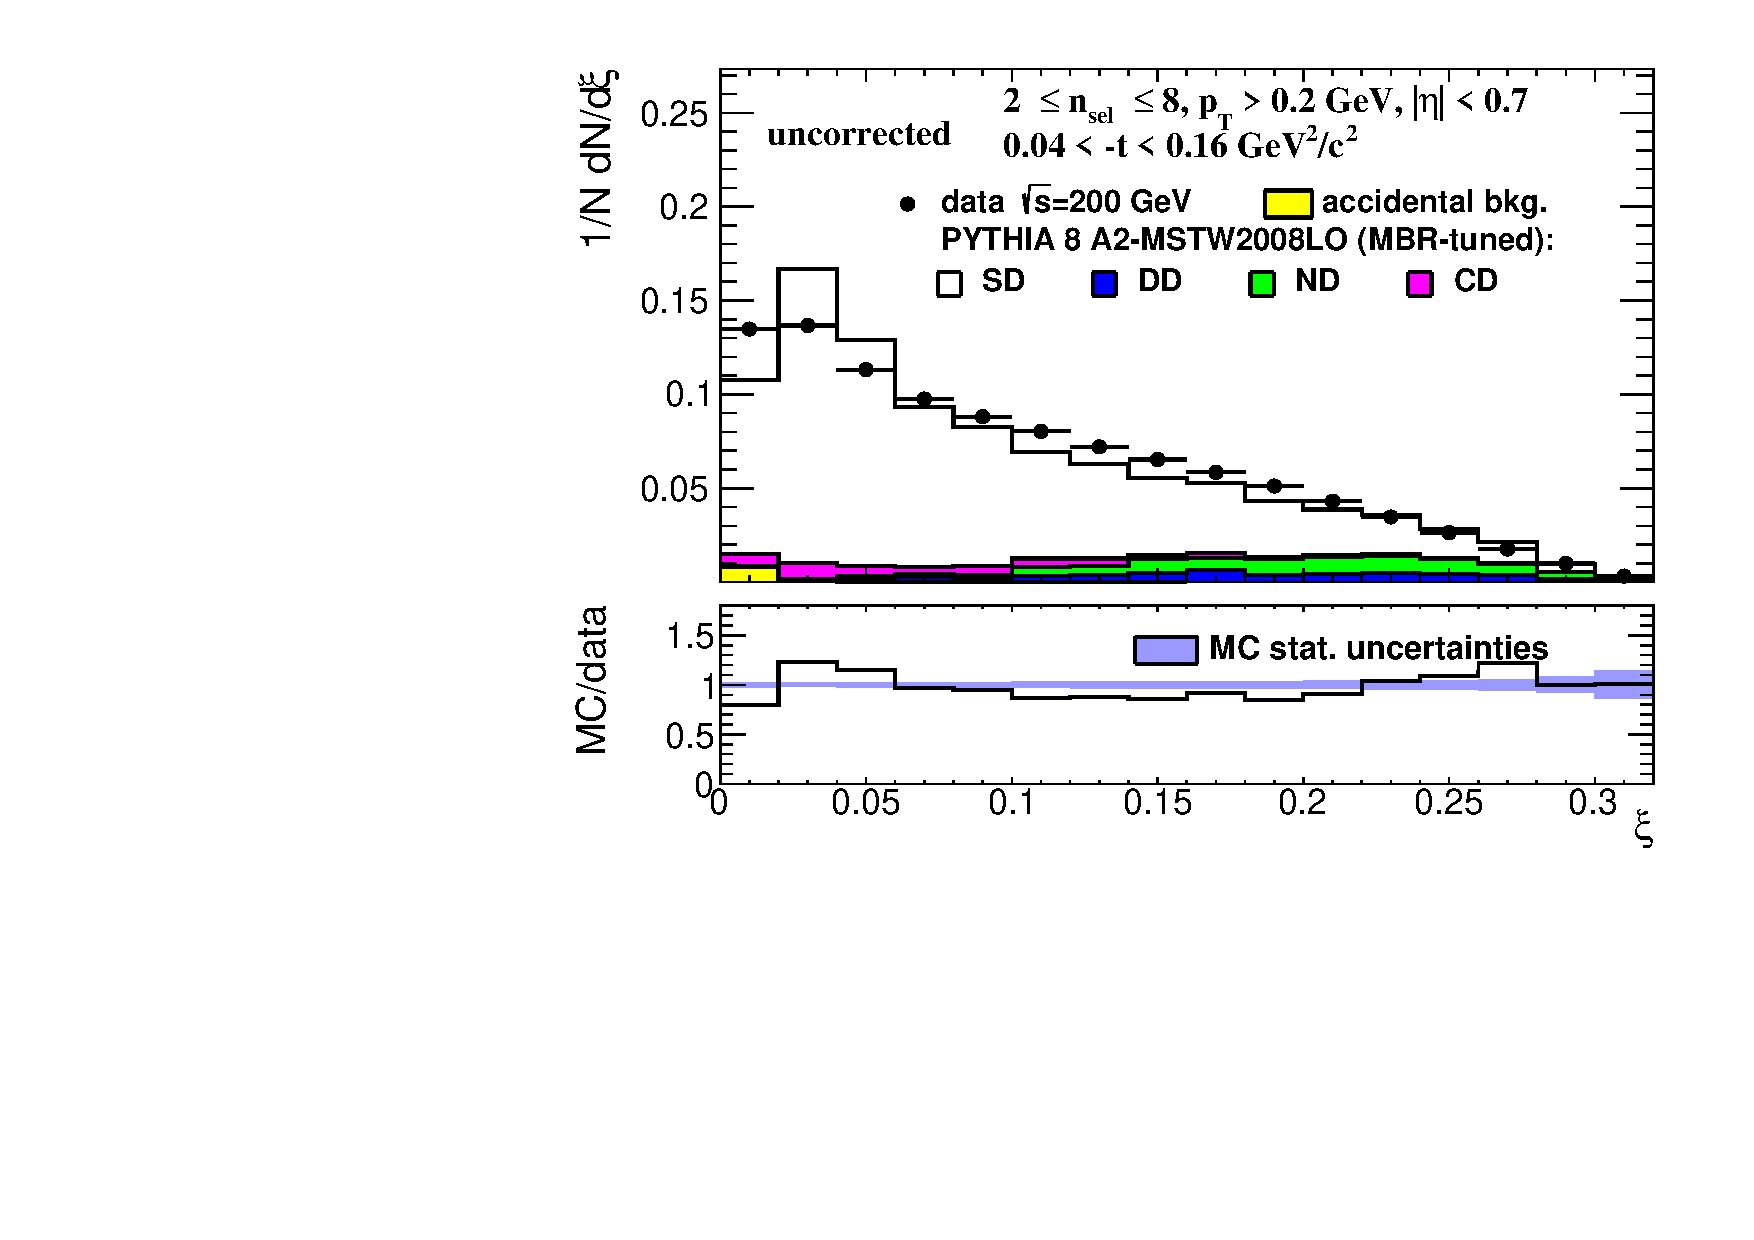
\includegraphics[width=.49\textwidth,page=1]{chapters/chrgSTAR/img/nonSD/SDT_pythia_xi0_option2_RP_starsim_xi.pdf}
	\hfill
	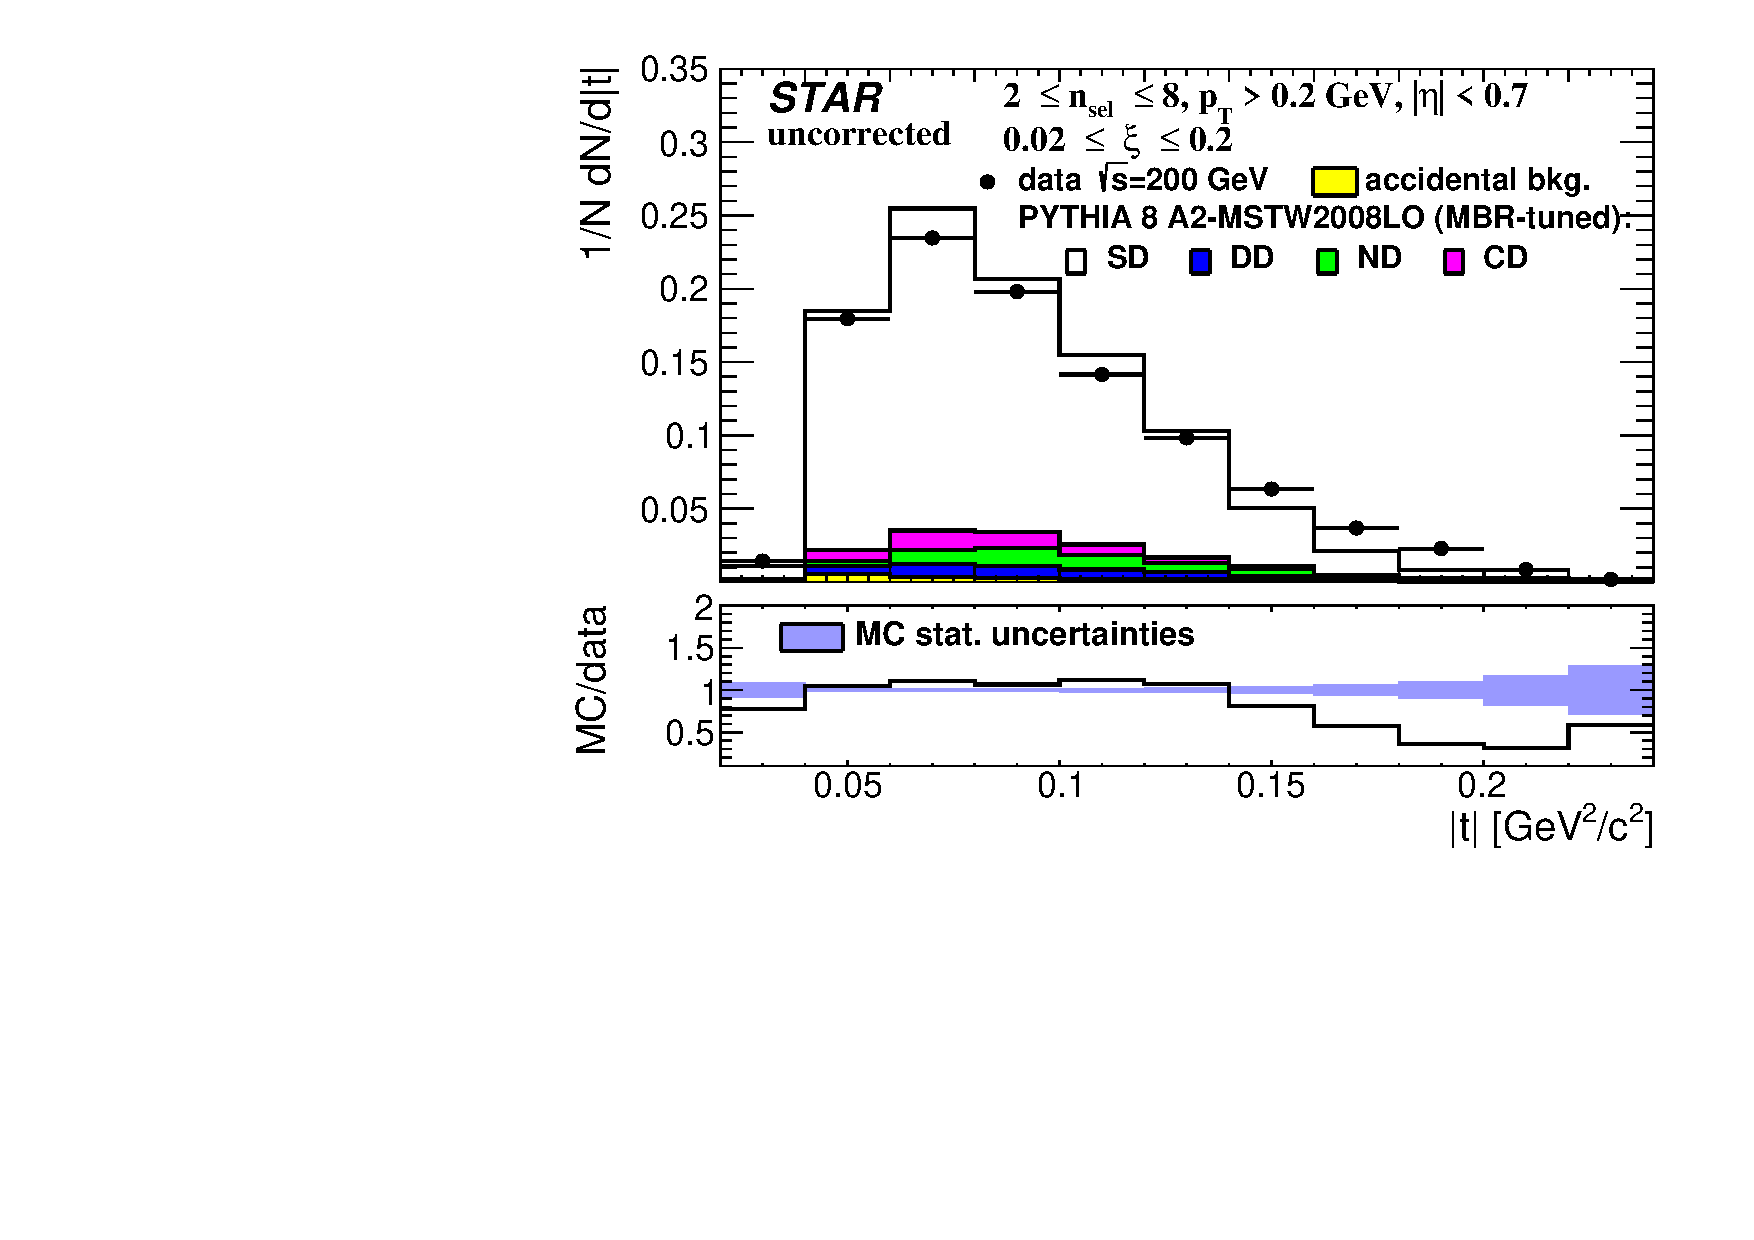
\includegraphics[width=.49\textwidth,page=1]{chapters/chrgSTAR/img/nonSD/SDT_pythia_xi0_option2_RP_starsim_t.pdf}
	\newline
	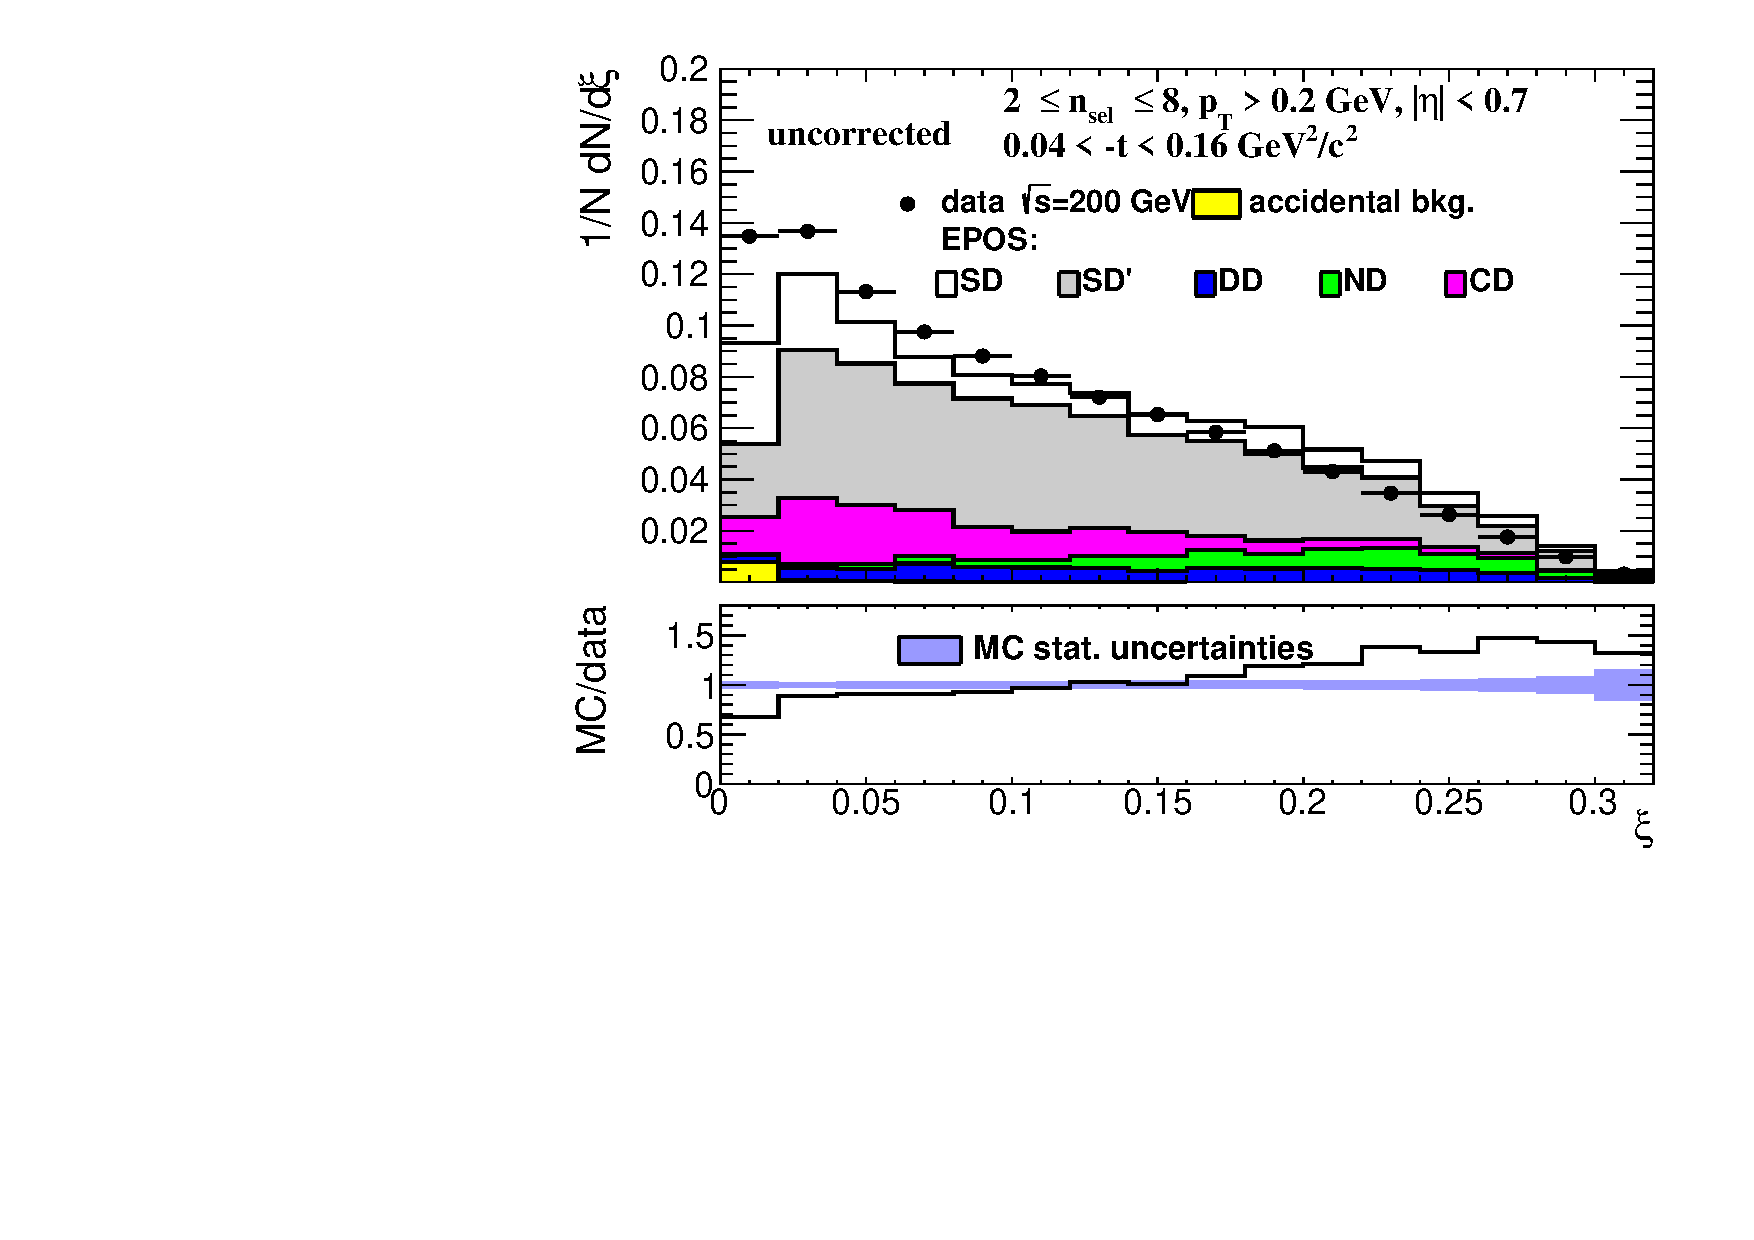
\includegraphics[width=.49\textwidth,page=1]{chapters/chrgSTAR/img/nonSD/SDT_epos_xi0_RP_starsim_xi.pdf}
	\hfill
	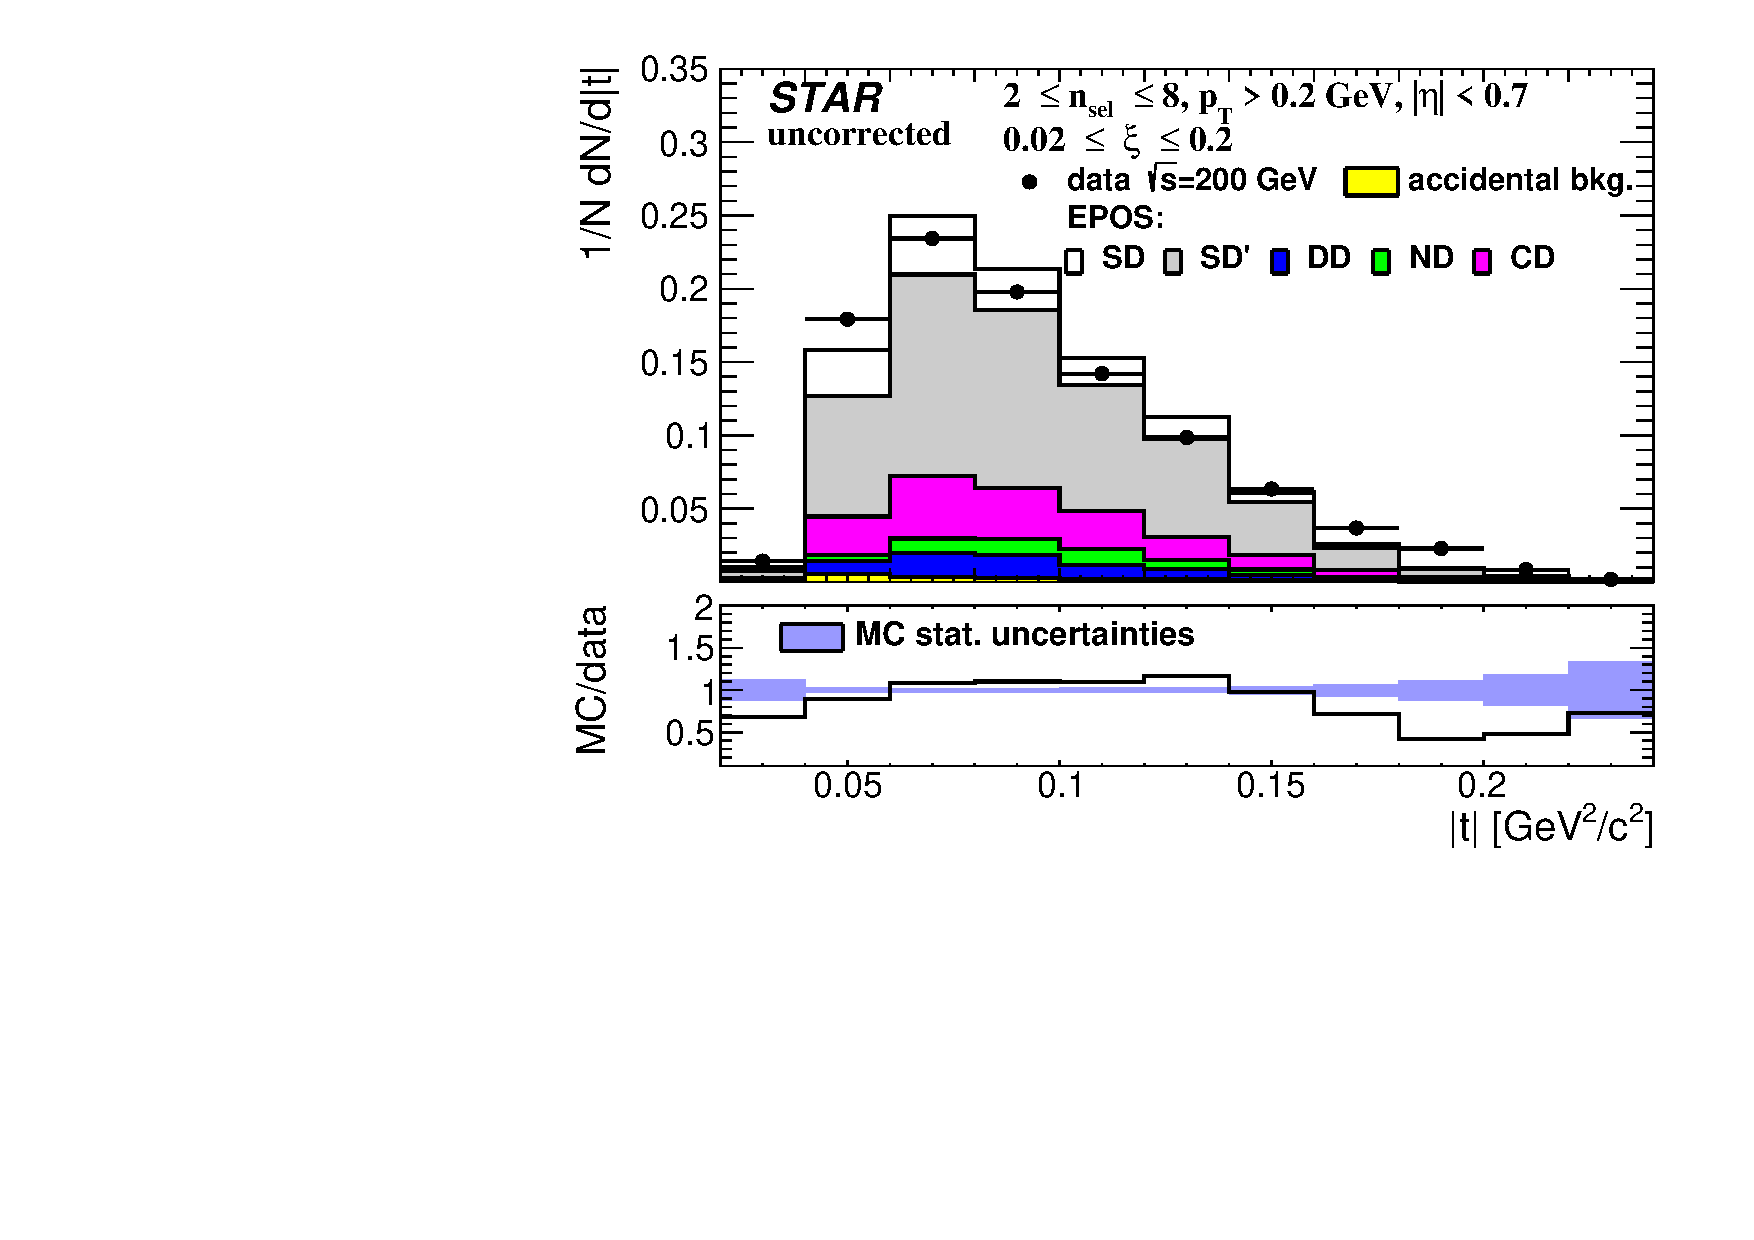
\includegraphics[width=.49\textwidth,page=1]{chapters/chrgSTAR/img/nonSD/SDT_epos_xi0_RP_starsim_t.pdf}
	%
	\caption{Uncorrected distributions of data compared to various MC models: (top) PYTHIA8 A2 (MBR), (middle) PYTHIA8 A2 (MBR-tuned) and (bottom) EPOS, as a function of (left column) $\xi$  and (right column) $|t|$.}
	\label{fig:nonSDxit}
	\vspace{-1.5cm}
\end{figure}
%\newpage

\begin{figure}[h!]
	\centering
	\begin{subfigure}{.49\textwidth}
		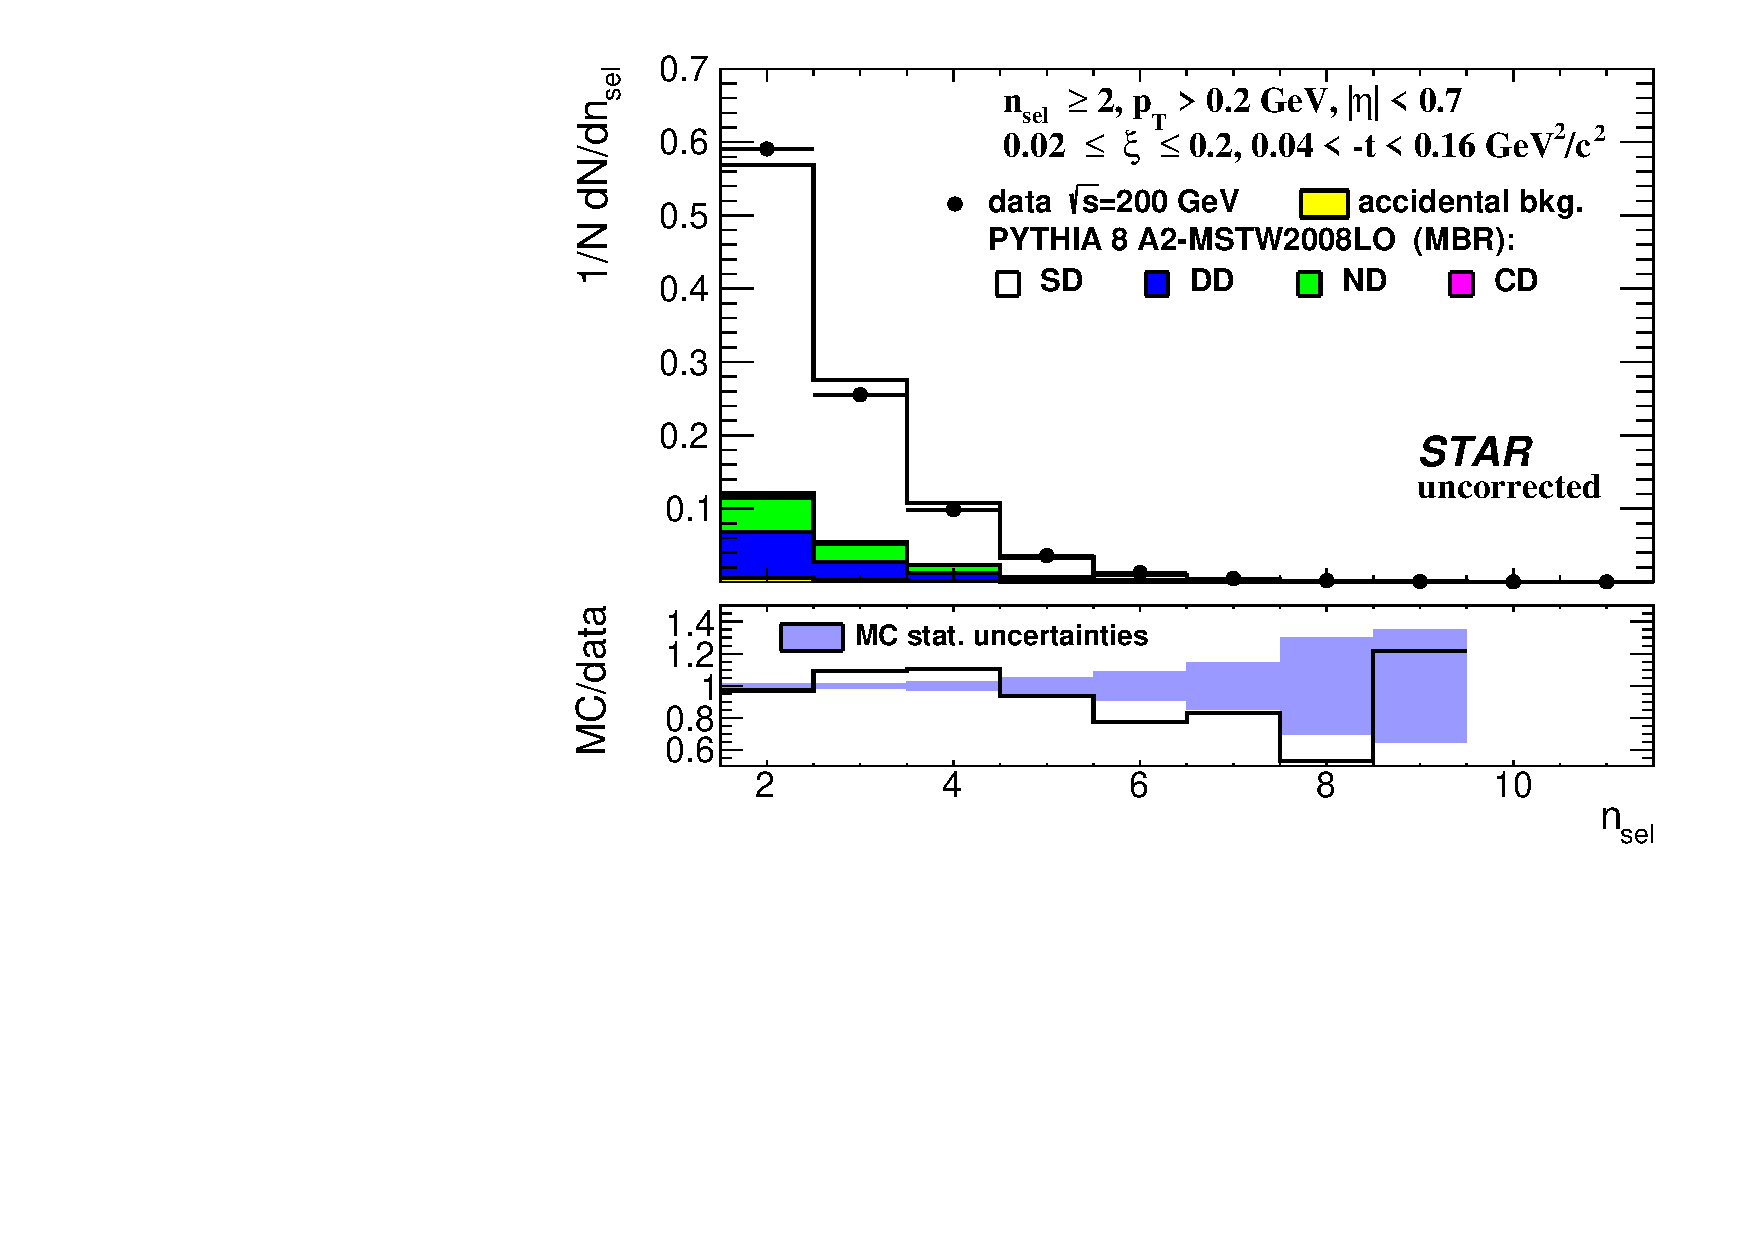
\includegraphics[width=\linewidth, page=1]{chapters/chrgSTAR/img/nonSD/chrg/SDT_pythia_xi0_RP_starsim_nsel.pdf}
	\end{subfigure}
	\begin{subfigure}{.49\textwidth}
		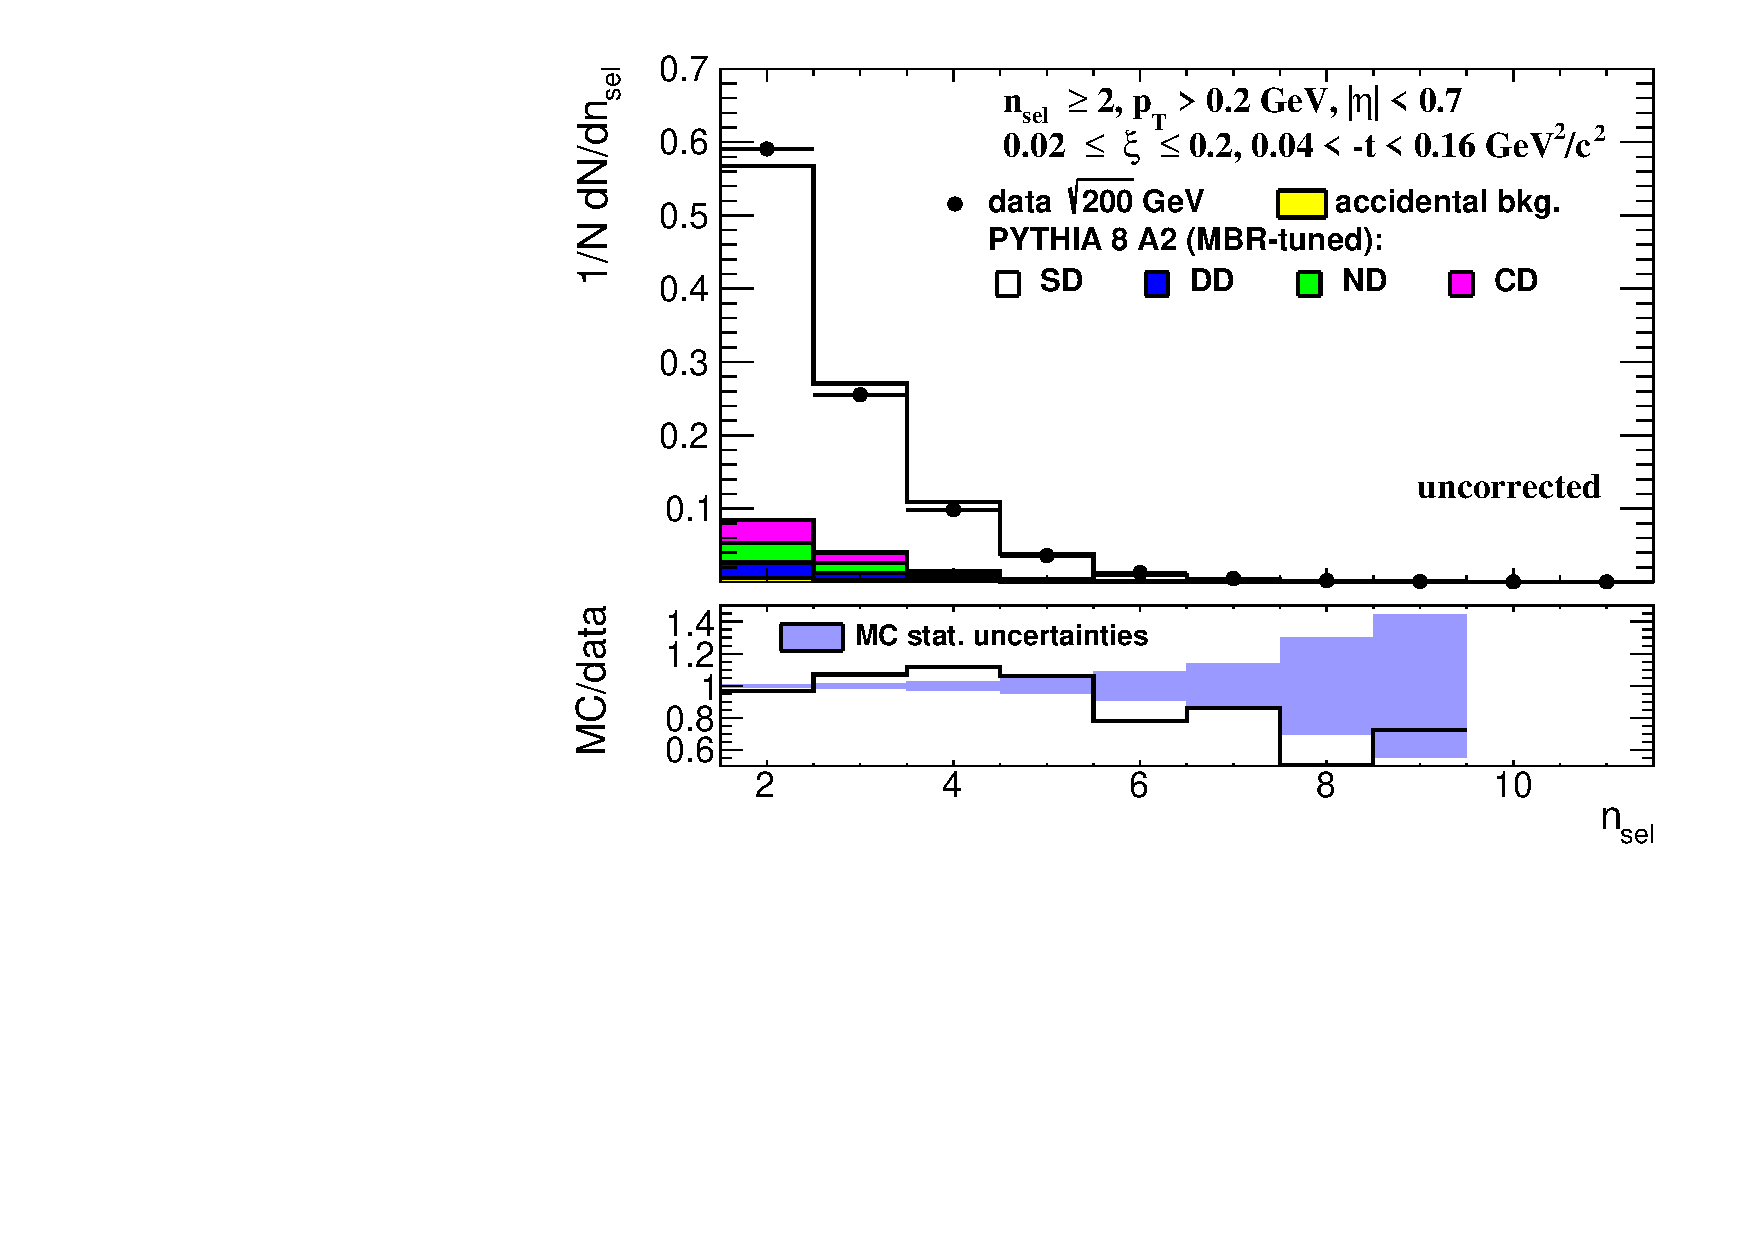
\includegraphics[width=\linewidth, page=1]{chapters/chrgSTAR/img/nonSD/chrg/SDT_pythia_xi0_option2_RP_starsim_nsel.pdf}
	\end{subfigure}
	\begin{subfigure}{.49\textwidth}
		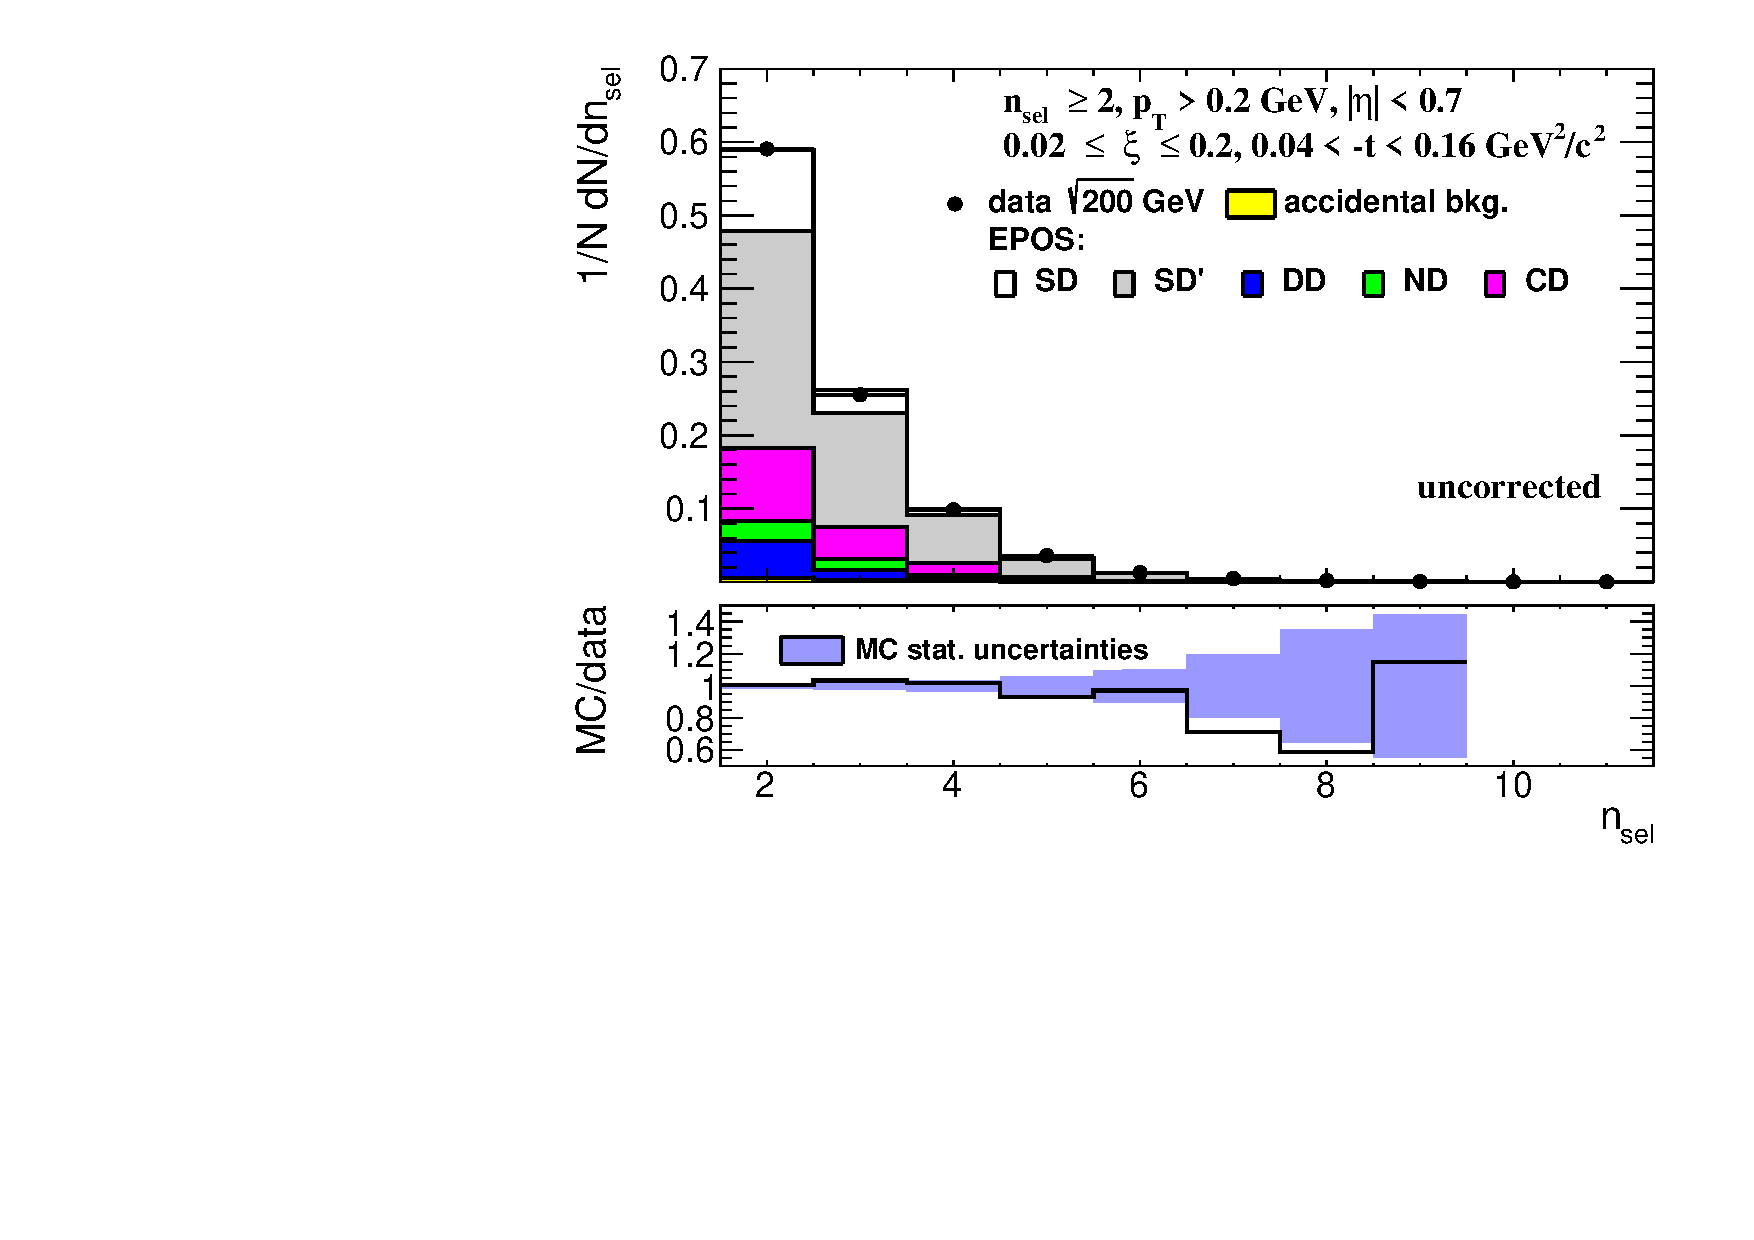
\includegraphics[width=\linewidth, page=1]{chapters/chrgSTAR/img/nonSD/chrg/SDT_epos_xi0_RP_starsim_nsel.pdf}
	\end{subfigure}
	\begin{minipage}{.49\textwidth}
		\caption{Uncorrected distributions of data compared to various MC models: (top left) PYTHIA8 A2 (MBR), (top right) PYTHIA8 A2 (MBR-tuned) and (bottom) EPOS, as a function of $n_{\mathrm{sel}}$.}
		\label{fig:nonSDnsel}
	\end{minipage}
	
\end{figure}
\begin{figure}[h!]
%	\vspace{-0.5cm}
	\centering
	\begin{subfigure}{.49\textwidth}
		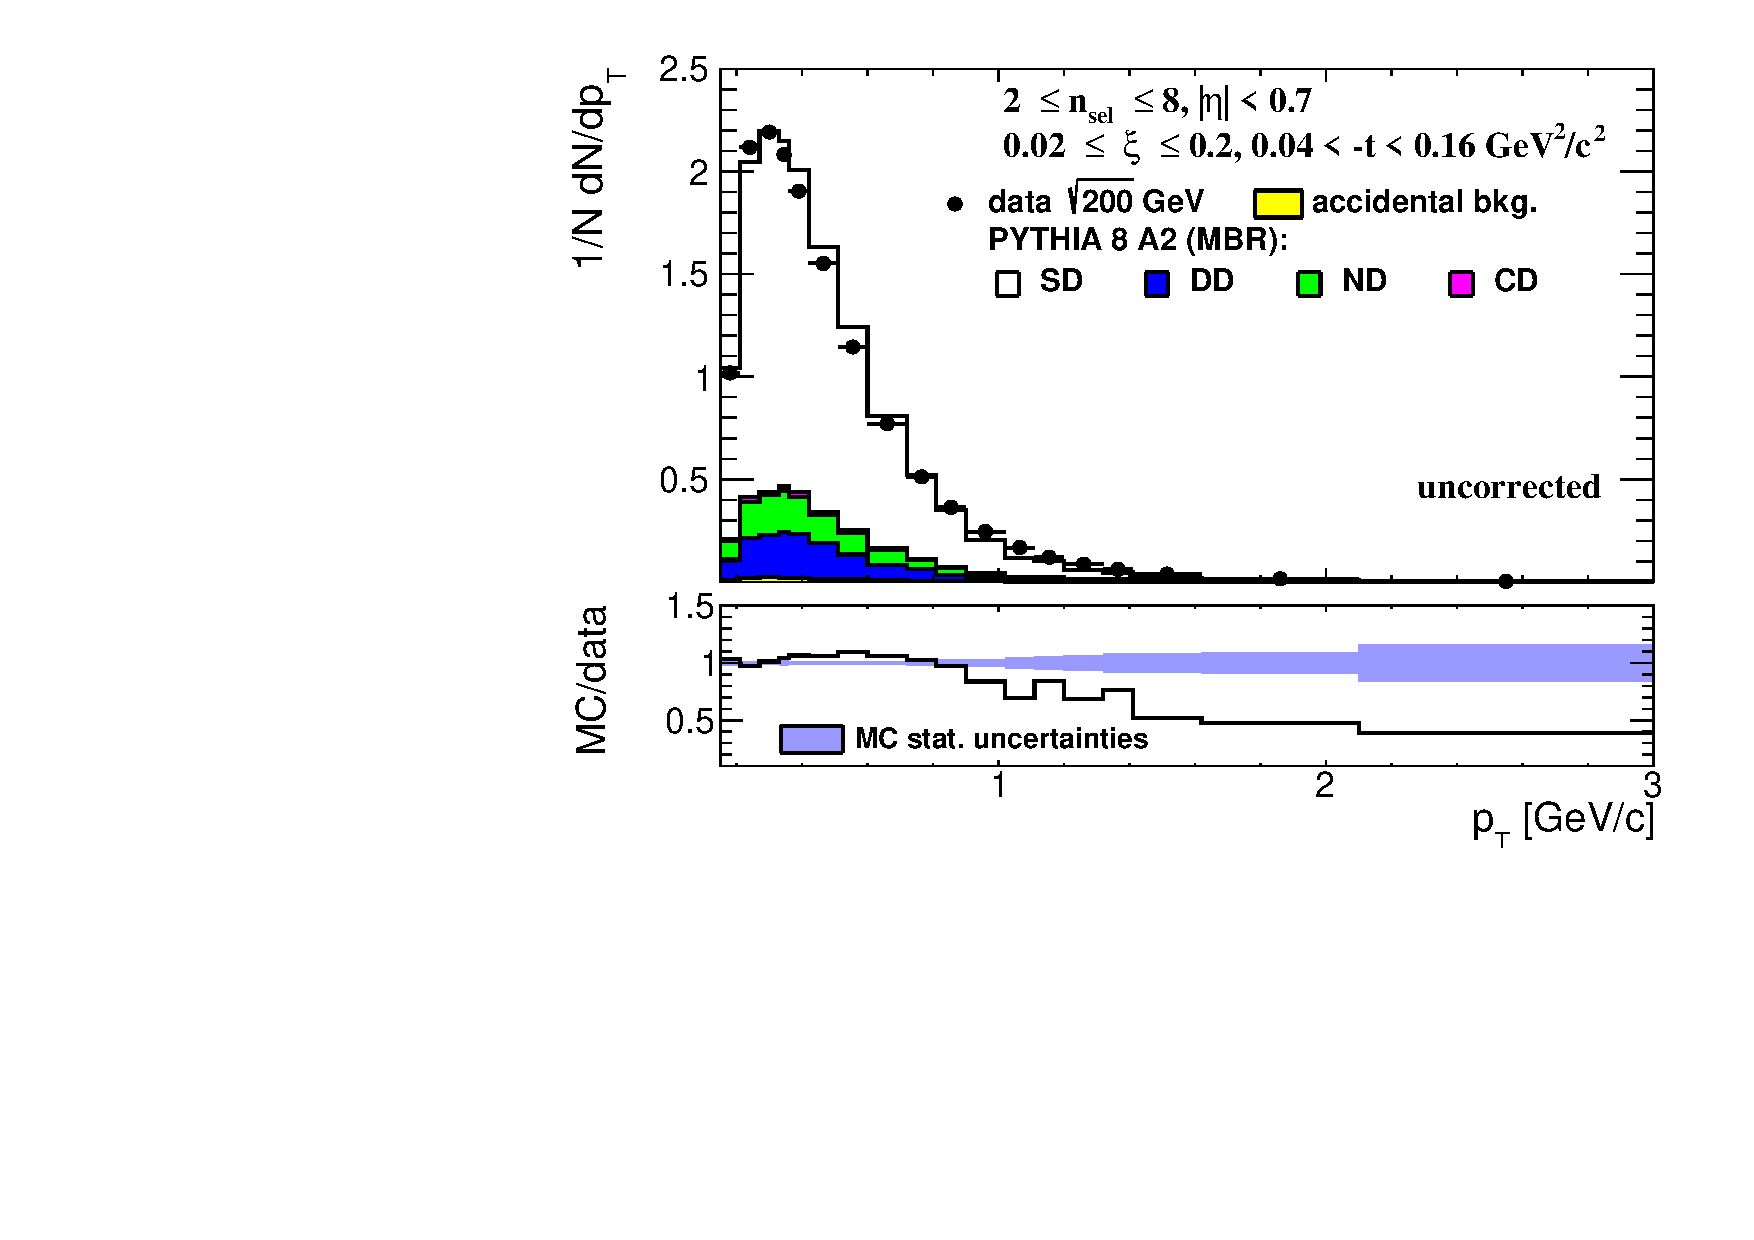
\includegraphics[width=\linewidth, page=1]{chapters/chrgSTAR/img/nonSD/chrg/SDT_pythia_xi0_RP_starsim_pt.pdf}
	\end{subfigure}
	\begin{subfigure}{.49\textwidth}
		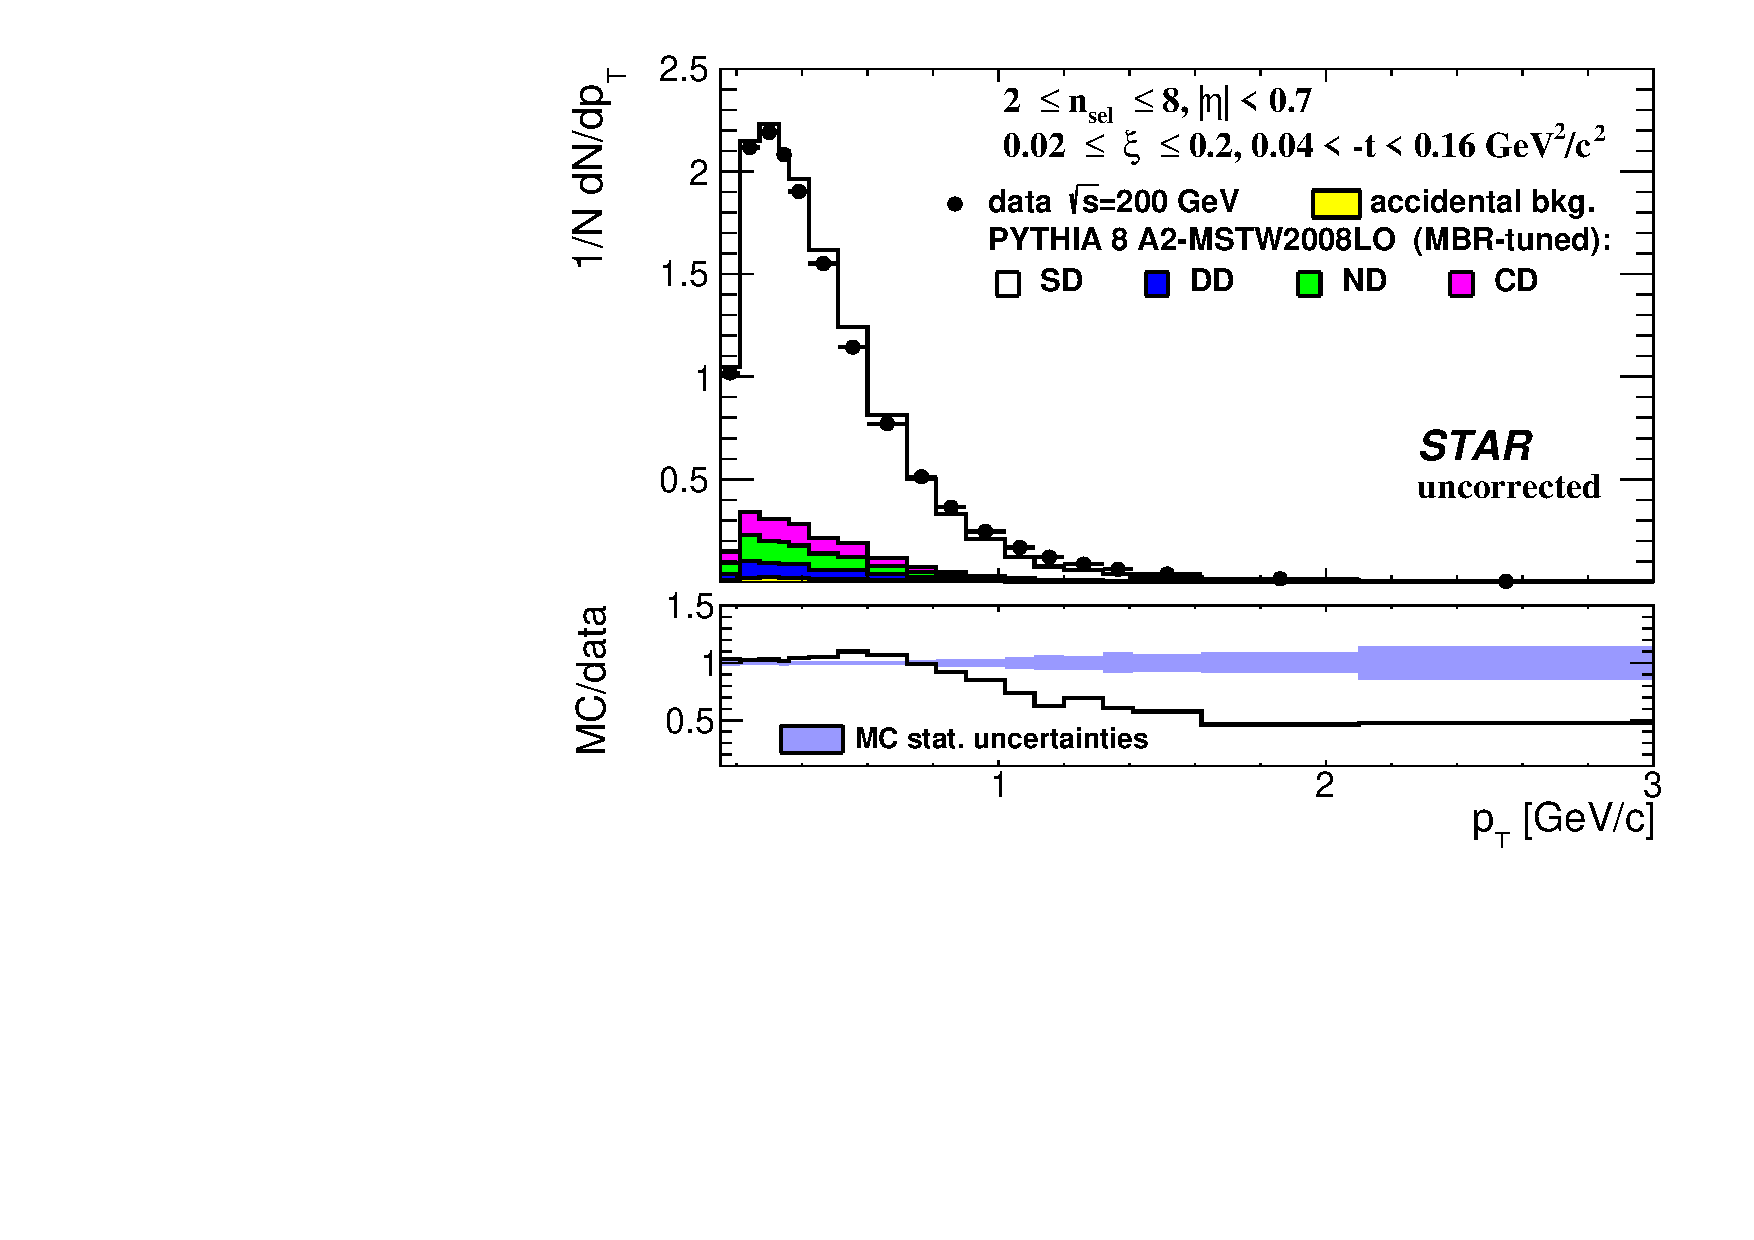
\includegraphics[width=\linewidth, page=1]{chapters/chrgSTAR/img/nonSD/chrg/SDT_pythia_xi0_option2_RP_starsim_pt.pdf}
	\end{subfigure}
	\begin{subfigure}{.49\textwidth}
		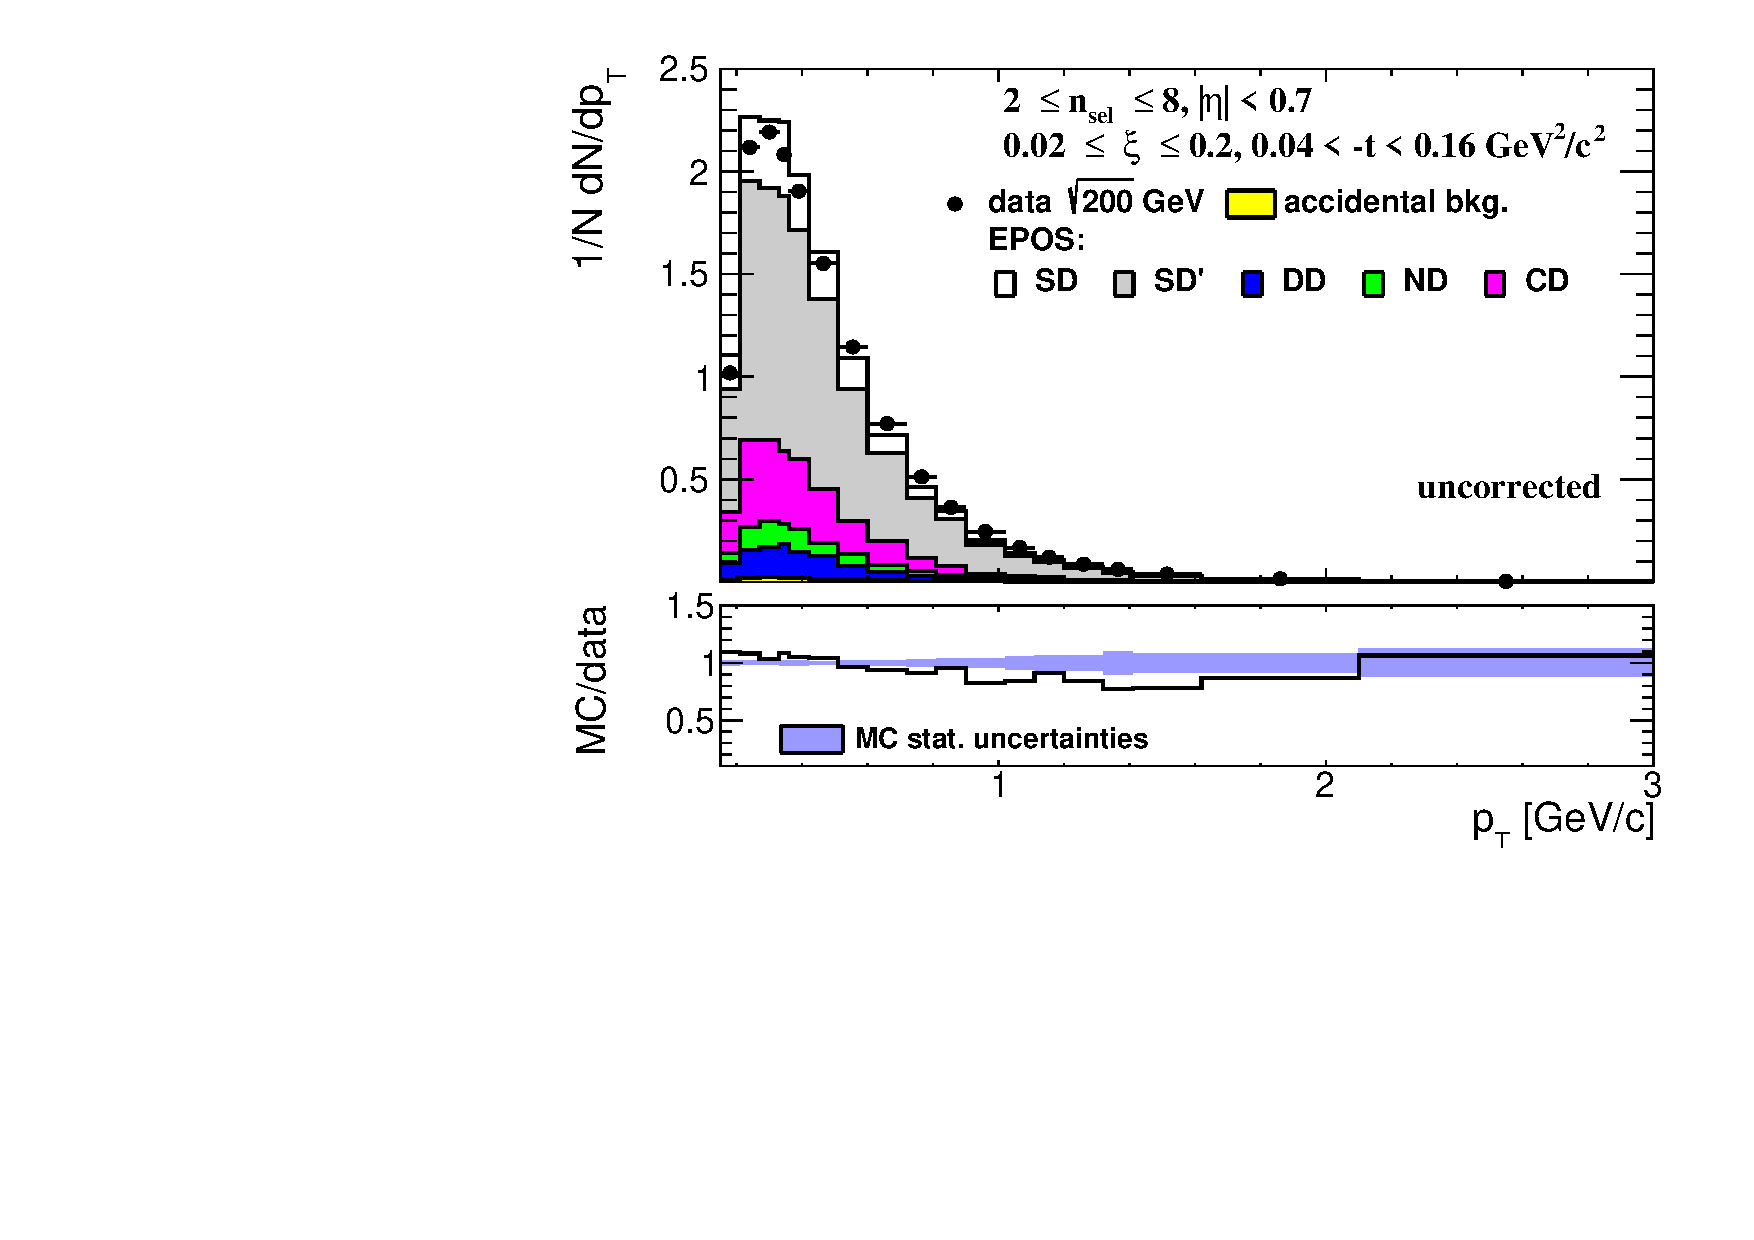
\includegraphics[width=\linewidth, page=1]{chapters/chrgSTAR/img/nonSD/chrg/SDT_epos_xi0_RP_starsim_pt.pdf}
	\end{subfigure}
	\begin{minipage}{.49\textwidth}
		\caption{Uncorrected distributions of data compared to various MC models: (top left) PYTHIA8 A2 (MBR), (top right) PYTHIA8 A2 (MBR-tuned) and (bottom) EPOS, as a function of $p_{\mathrm{T}}$.}
		\label{fig:nonSDpt}
	\end{minipage}
	
\end{figure}
%\newpage
\begin{figure}[h!]
%	\vspace{-0.5cm}
	\centering
	\begin{subfigure}{.49\textwidth}
		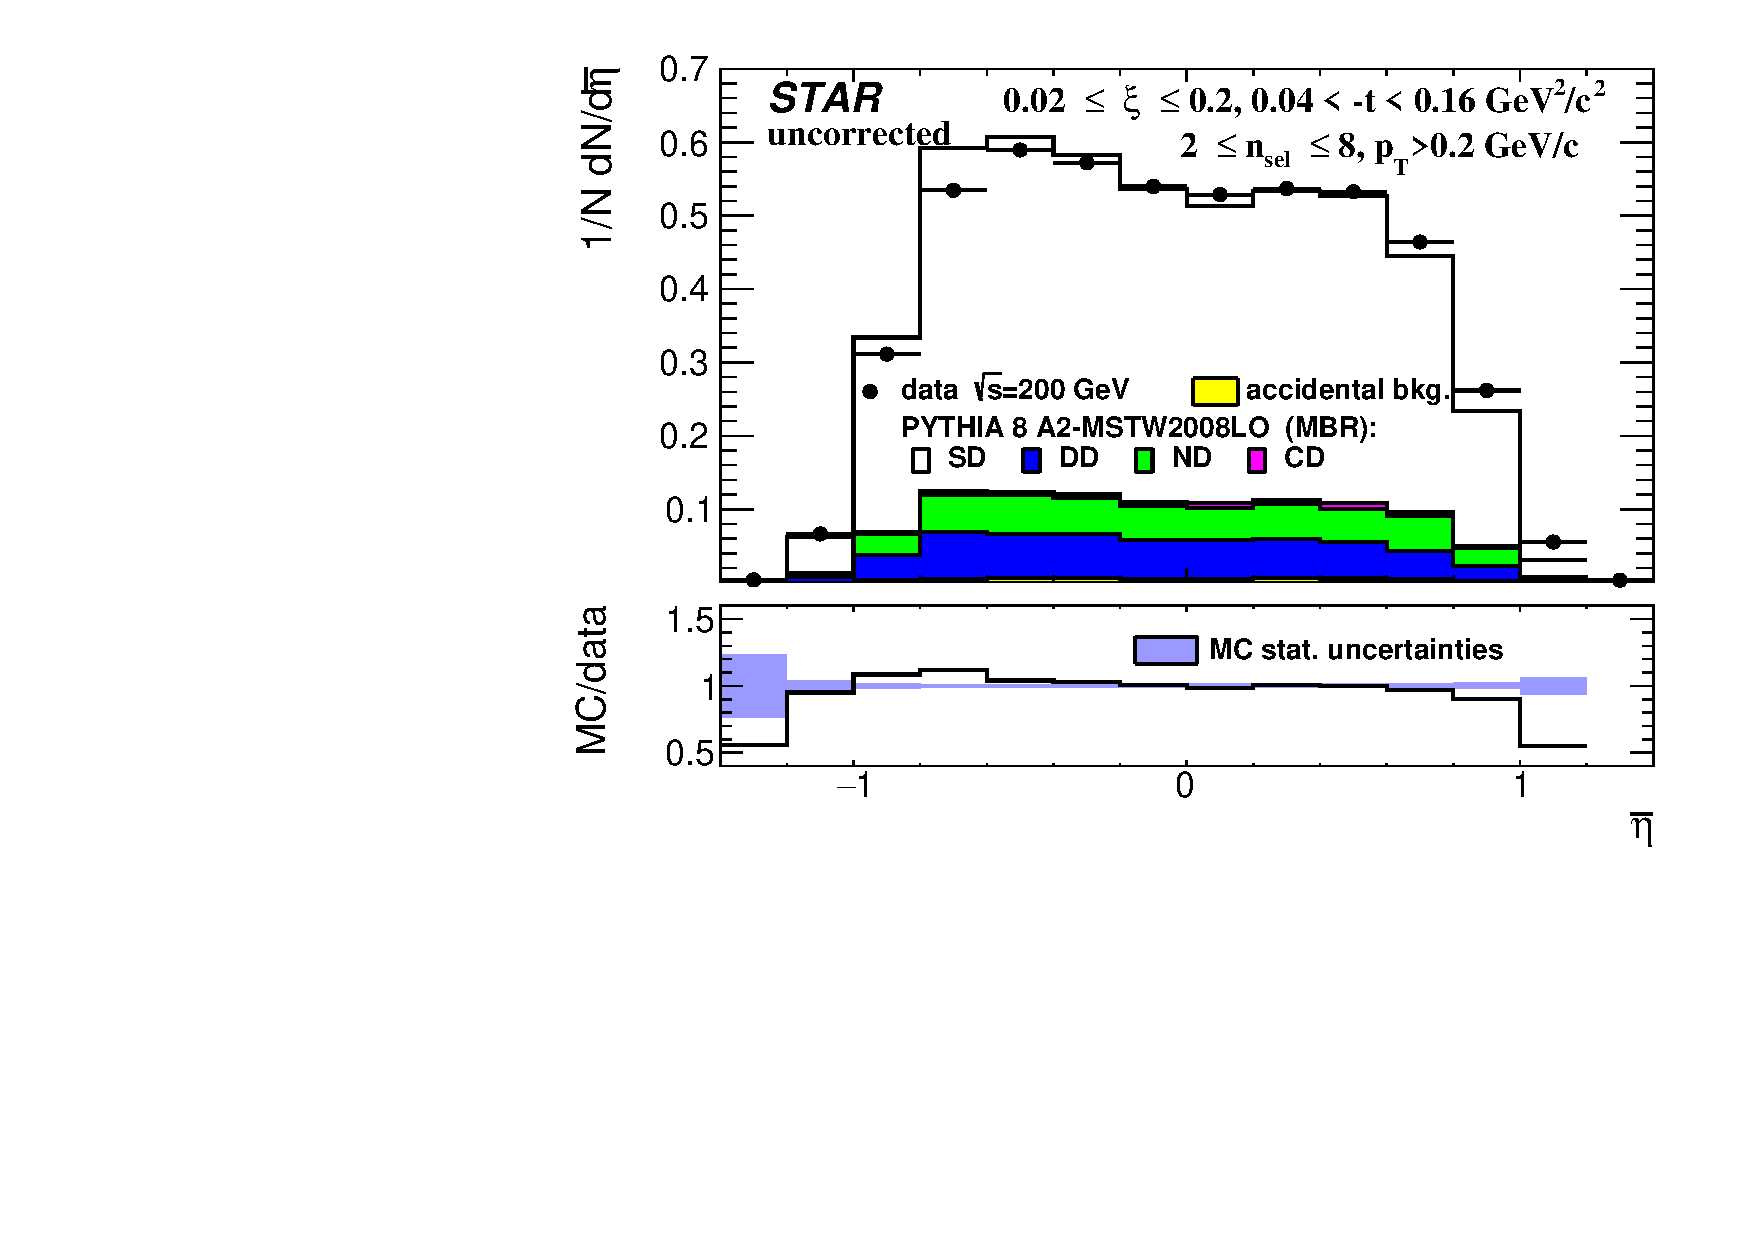
\includegraphics[width=\linewidth, page=1]{chapters/chrgSTAR/img/nonSD/chrg/SDT_pythia_xi0_RP_starsim_eta.pdf}
	\end{subfigure}
	\begin{subfigure}{.49\textwidth}
		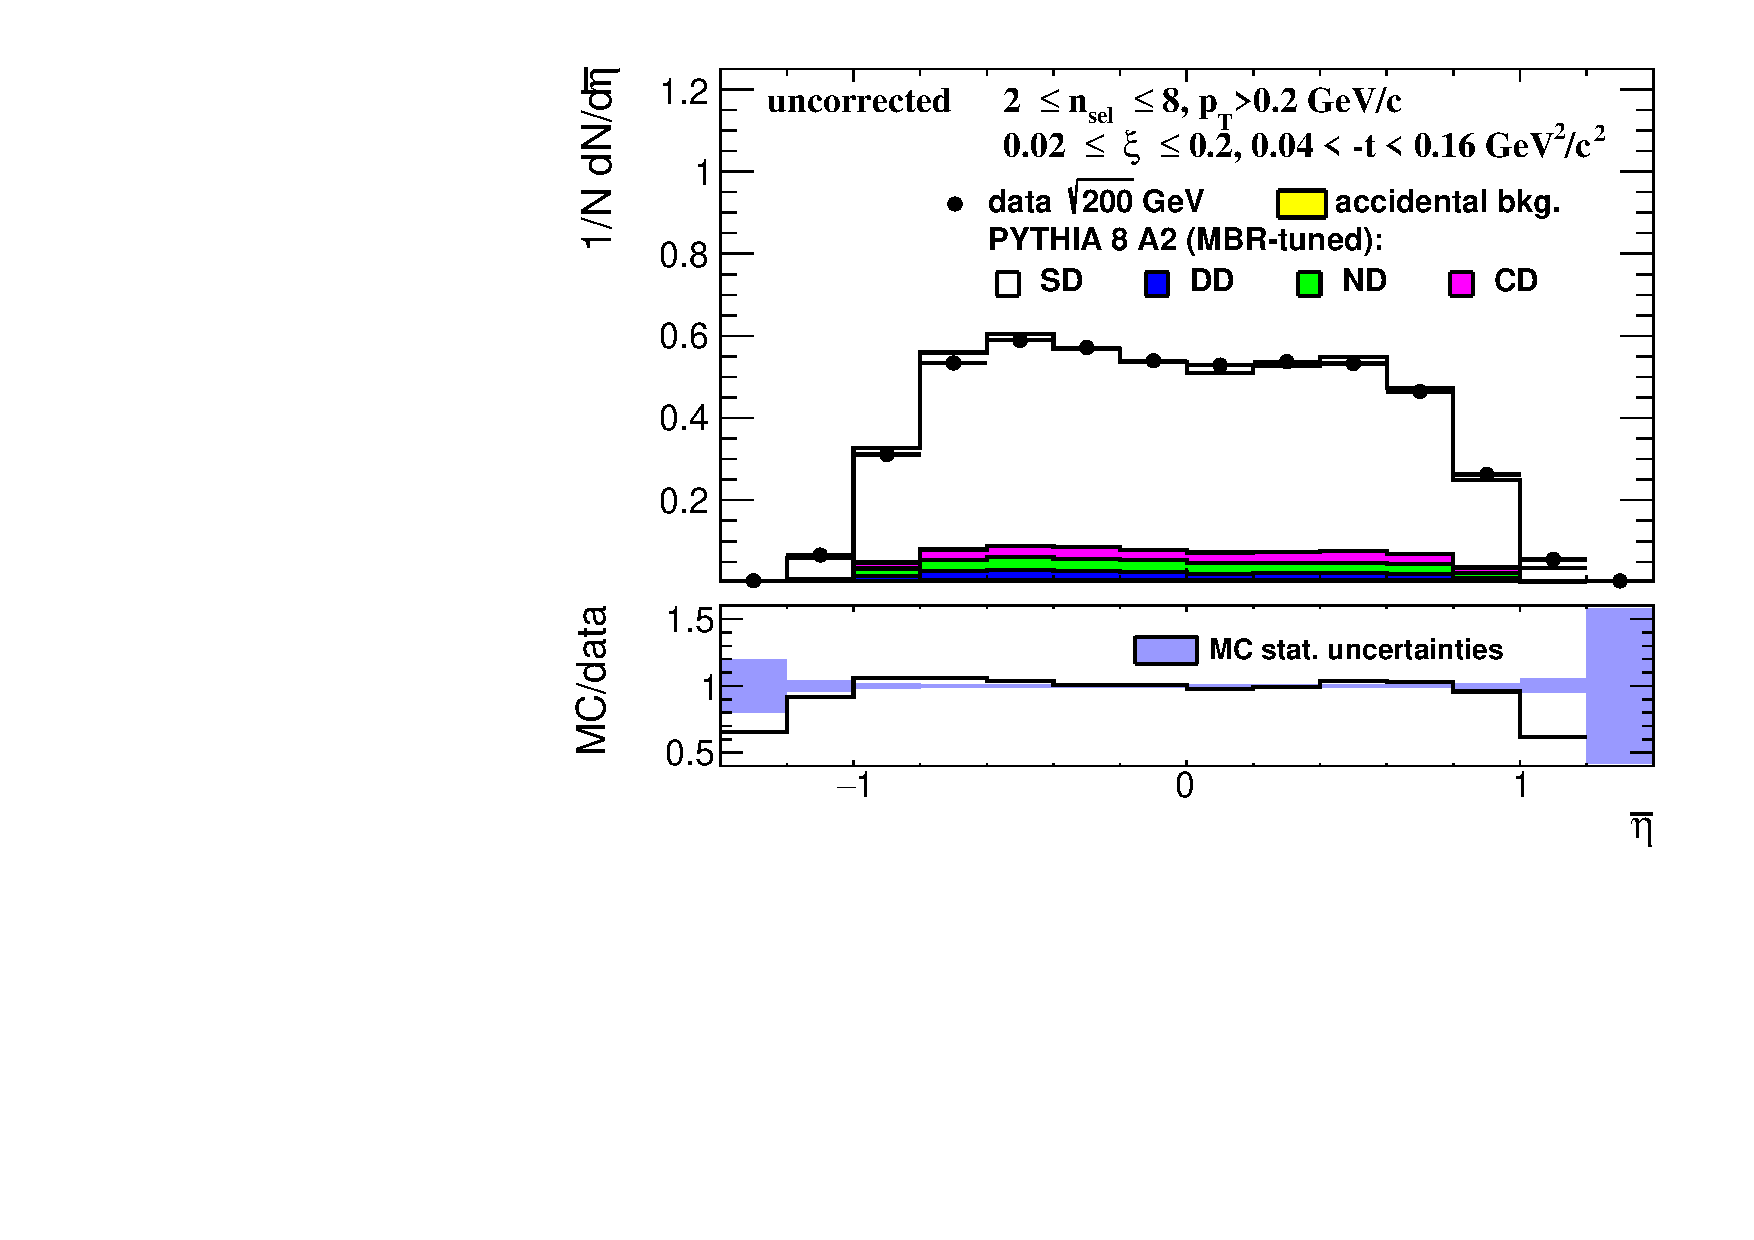
\includegraphics[width=\linewidth, page=1]{chapters/chrgSTAR/img/nonSD/chrg/SDT_pythia_xi0_option2_RP_starsim_eta.pdf}
	\end{subfigure}
	\begin{subfigure}{.49\textwidth}
		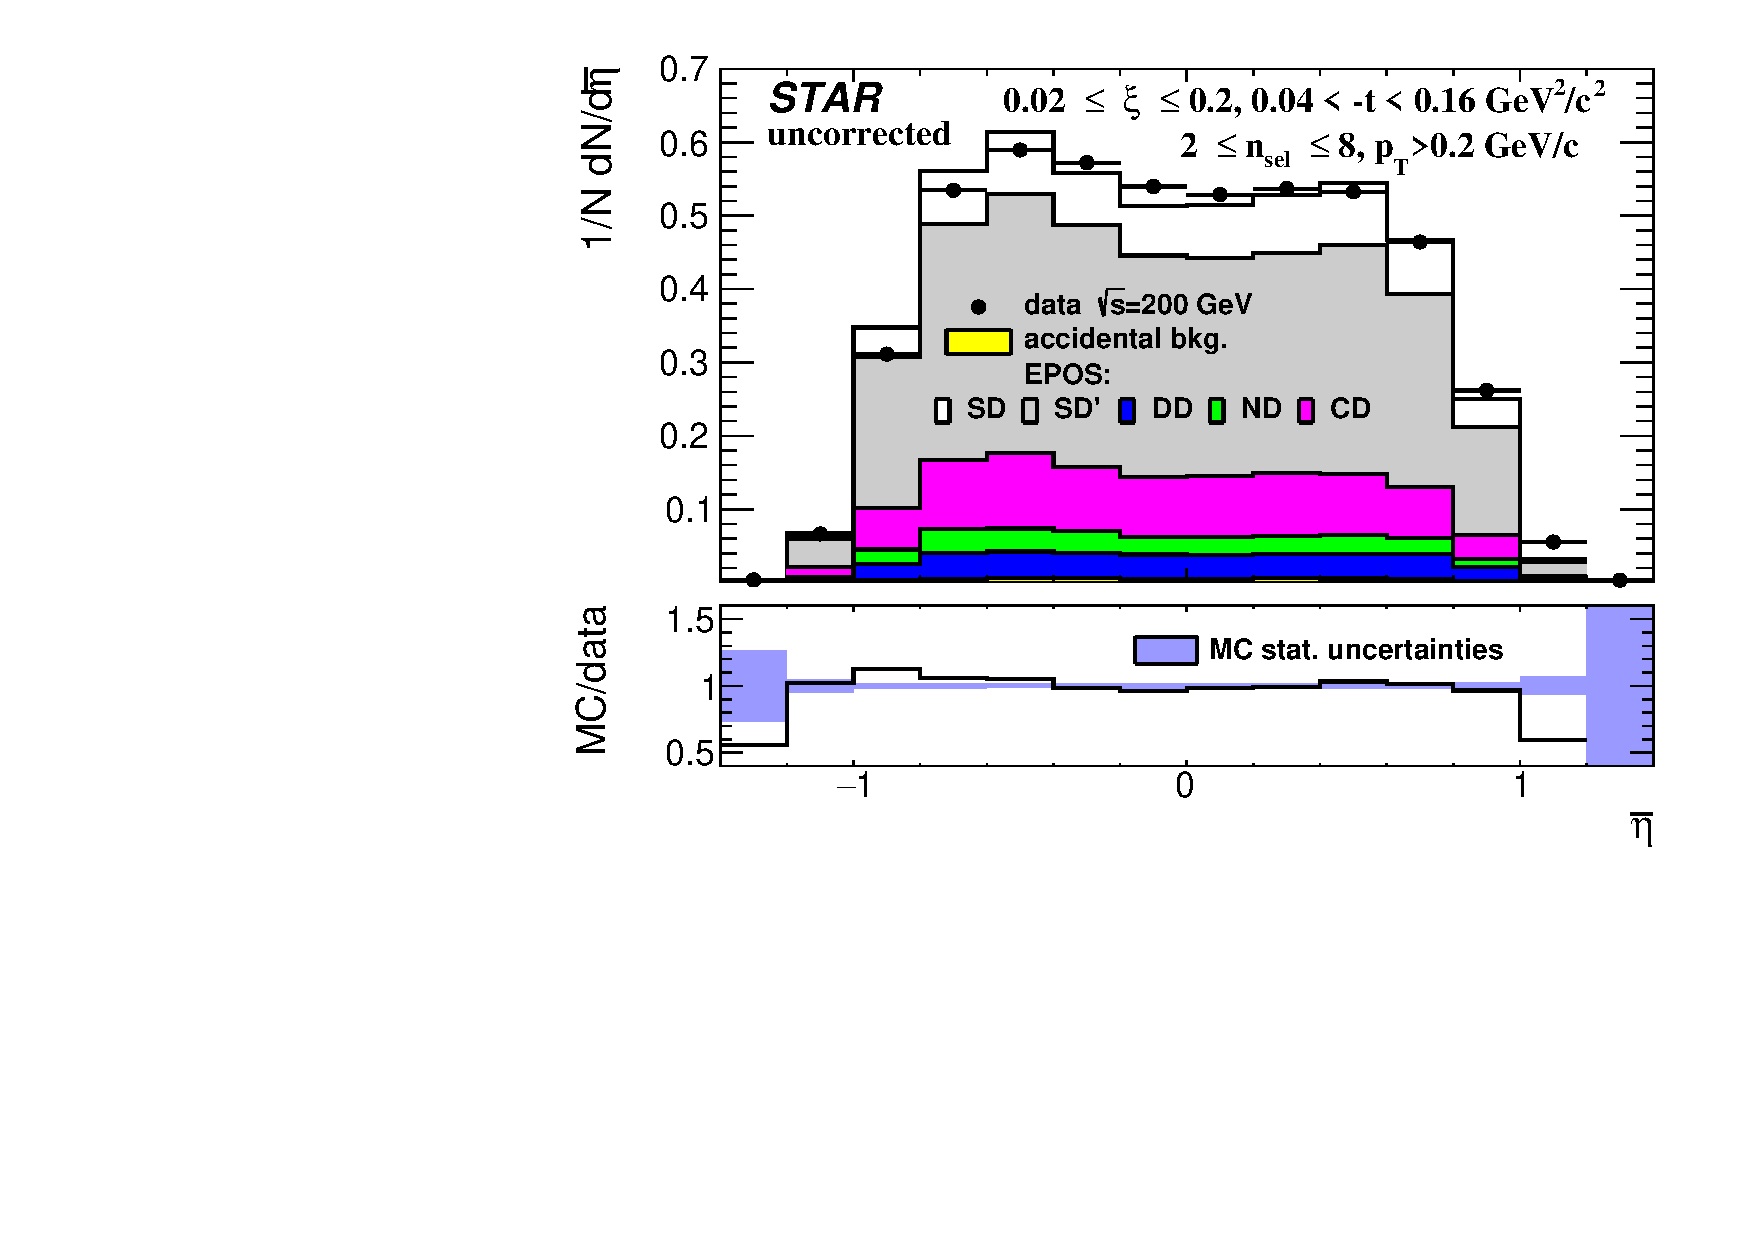
\includegraphics[width=\linewidth, page=1]{chapters/chrgSTAR/img/nonSD/chrg/SDT_epos_xi0_RP_starsim_eta.pdf}
	\end{subfigure}
	\begin{minipage}{.49\textwidth}
		\caption{Uncorrected distributions of data compared to various MC models: (top left) PYTHIA8 A2 (MBR), (top right) PYTHIA8 A2 (MBR-tuned) and (bottom) EPOS, as a function of $\bar{\eta}$. }
		\label{fig:nonSDera}
	\end{minipage}
	
\end{figure}
\FloatBarrier